\section{\textit{session-rec}} A biblioteca \textit{session-rec} foi
desenvolvida para facilitar experimentos comparando recomendadores
\textit{session-based} em Python. A biblioteca contém as implementações dos
modelos previamente citados no presente trabalho. Um novo modelo pode ser
implementado seguindo o polimorfismo das demais implementações.

Cada experimento é declarado em um arquivo .yml, contendo as informações dos
dados a serem utilizados, dos modelos a serem avaliados e de seus hiperparâmetros.

A biblioteca contém um script de pré--processamento, responsável por separar os
dados em conjuntos de treinamento, validação e teste, filtrando os dados de
acordo com o suporte mínimo dos itens e o número mínimo de usuários por sessão,
à escolha do usuário. Em geral, os conjuntos de testes nos comparativos
publicados utilizando a ferramenta é limitado a itens nos dias mais recentes, da
ordem de 1 a 7 dias.

A divisão dos dados pode ser feita de duas formas: \textit{single split} e
\textit{window}. A primeira forma divide o conjunto de dados em um único
conjunto de teste e treinamento. A segunda forma divide a base de dados em
múltiplos conjuntos de acordo com uma janela de tempo especificada. Dessa forma, os
últimos dias de cada conjunto são reservados para teste, enquanto que os dias
anteriores da mesma janela são utilizados para o treinamento.

 Entre os métodos de avaliação disponíveis na biblioteca, há dois mais
 utilizados em publicações com os comparativos: no primeiro, avalia-se a
 capacidade de prever o próximo item imediato da sessão. No segundo, avalia-se a
 capacidade de prever todos os itens subsequentes da sessão.

 O presente trabalho utiliza também uma terceira forma de avaliação, em que
 avalia-se apenas o último item da sessão.

\section{Análise preliminar dos dados}

Os dados utilizados neste trabalho consistem nas sessões de gravação no
Indaband, no período compreendido entre 01 de janeiro de 2023 até 19 de dezembro
de 2023.


\begin{table}[H]
  \centering
  \begin{tabular}{|l|l|}
    \hline
    \textbf{Período} & 01/01/2023 a 19/12/2023 \\ \hline
    Sessões criadas & 93.314 \\ \hline
    Sessões publicadas & 18.845 \\ \hline
    Usuários que adicionaram faixas & 11.968 \\ \hline
    Usuários com faixas publicadas & 3.630 \\ \hline
    Faixas adicionadas & 457.224 \\ \hline
    Faixas \textit{forkadas} & 349.060 \\ \hline
    Faixas publicadas & 134.004 \\ \hline
  \end{tabular}
  \caption{Quantidade de sessões, faixas e usuários no período de 01/01/2023 a 19/12/2023.}
  \label{tab_sessoes}
\end{table}

Verifica-se na tabela \ref{tab_sessoes} uma grande quantidade de faixas criadas,
\textit{forkadas} e publicadas na plataforma. Essas faixas são criadas por um
número pequeno de usuários. Por sua vez, na tabela \ref{tab_convites}, a
quantidade de convites enviados e aceitos é ainda menor em relação ao número de
usuários ativos no período.

\begin{table}[htbp]
  \centering
  \begin{tabular}{|l|l|}
    \hline
    \textbf{Período} & 01/01/2023 a 19/12/2023 \\ \hline
    Sessões criadas & 93.315 \\ \hline
    Sessões com convites & 3.984 \\ \hline
    Sessões com participantes & 1.388 \\ \hline
    Convites & 4.619 \\ \hline
    Convites aceitos & 2.799 \\ \hline
    Usuários que convidaram & 592 \\ \hline
    Usuários convidados & 934 \\ \hline
    Usuários que aceitaram convites & 652 \\ \hline
  \end{tabular}
  \caption{Informações sobre convites no período de 01/01/2023 a 19/12/2023.}
  \label{tab_convites}
\end{table}

Em razão desses dois aspectos, o sistema de recomendação \textit{session-based}
proposto prevê qual o próximo usuário cuja faixa será incluída na sessão, dados
os demais usuários com faixas inclusas e do histórico de sessões dos usuários
envolvidos. Por mais que essa abordagem não utilize os convites, ela é capaz de
recomendar usuários que ainda não tenham contribuído para a sessão e que
potencialmente possam contribuir.

Dessa forma, os itens das sessões serão os próprios usuários, e não as faixas,
evitando que o sistema recomende um usuário que já tenha uma faixa incluída na
sessão. Além disso, seguindo a abordagem \textit{session-aware}, o criador de
cada sessão será considerado como o usuário ativo, ou seja, o usuário que
receberá as recomendações. Isso permite que o sistema modele as preferências
individuais de usuários ao criarem sessões.

% Em razão da modelagem apresentada, os padrões mais esperados para os modelos são:

% \begin{itemize}
%   \item Usuários que co-participem de sessões e tendem a repetir as
%   colaborações serem previstos corretamente como próximo usuário e recomendados;
%   \item Sessões com muitos \textit{forks} sejam mais fáceis de prever o próximo
%   usuário e os usuários restantes, uma vez que a base de dados contém diferentes
%   variações dessas sessões e de seus \textit{forks};
%   \item Na abordagem \textit{session-based}, a predição do último usuário da
% sessão erre mais do que a predição do próximo usuário e do que a dos
% usuários restantes, por tratar-se de um item inédito tanto naquela sessão quanto
% nas sessões precedentes no caso de um \textit{fork};
%   \item Que na abordagem \textit{session-based}, usuários que se isolam e que
%  praticam a partir de \textit{forks} de outros usuários, sem necessariamente
%  publicar suas versões, sejam previstos incorretamente como o próximo usuário
%  para sessões de outros usuários e recomendado -- o que não necessariamente
%  seria algo negativo, sob o ponto de vista de integrá-lo à comunidade -- e que esse
%  mesmo comportamento não seja observado na abordagem \textit{session-aware}, uma vez que 
%  há a informação do dono da sessão;
%   \item Na abordagem \textit{session-aware}, que os principais colaboradores de
%   determinado dono da sessão sejam recomendados, por mais que ambos não constem como
%   itens na sessão.
% \end{itemize}

 \section{Outros domínios}
 A seguir, são apresentadas as bases de dados utilizadas na bibliografia de
  SBRS. O domínio de cada uma dessas bases é de comércio eletrônico, música e
  notícias. Os valores das tabelas \ref{tab:datasets} e
  \ref{tab:datasets_comparison} foram retirados de \citet{ludewig_2018}.

  Observa-se que a base de dados do Indaband é a menor dentre as bases de dados
  disponíveis, considerando quantidade de interações, sessões e itens distintos.
  A quantidade menor de sessões e de valores diários se deve à recência da
  aplicação. A quantidade menor de itens por sessão se deve à modelagem do
  problema em que os itens são usuários distintos integrando cada sessão.
  É possível observar que algumas das bases contém taxas de interações e
  de itens únicos por sessão semelhantes às bases do Indaband.
  
  \begin{table}[htbp]
    \centering
    \begin{tabular}{lcccccc}
        \toprule
        \textbf{Dataset} & \textbf{RSC15-S} & \textbf{RSC15} & \textbf{TMALL} & \textbf{RETAILR} & \textbf{ZALANDO} \\
        \midrule
        Interações & 31.71M & 5.43M & 13.42M & 212.182 & 4.54M \\
        Sessões & 7.98M & 1.38M & 1.77M & 59.962 & 365.126 \\
        Itens & 37.483 & 28.582 & 425.348 & 31.968 & 189.328 \\
        Dias & 182 & 31 & 91 & 27 & 91 \\
        \hline
        Interações por sessão & 3,97 & 3,95 & 7,56 & 3,54 & 12,43 \\ 
        Itens únicos por sessão & 3,17 & 3,17 & 5,56 & 2,56 & 8,39 \\ 
        Interações por dia & 174,222 & 175,063 & 149,096 & 7,858 & 50,410 \\
        Sessões por dia & 43,854 & 44,358 & 19,719 & 2,220 & 4056 \\ 
        \bottomrule
    \end{tabular}
    \caption{Distribuição dos dados nos conjuntos de comércio eletrônico. O
    conjunto RSC15-S é a versão \textit{single-split} do conjunto RSC15. Os demais
    conjuntos são a média de 5 \textit{splits}. }
    \label{tab:datasets}
  \end{table}
  
  \begin{table}
    \centering
    \begin{tabular}{lcccccc}
        \toprule
        \textbf{Dataset} & \textbf{8TRACKS} & \textbf{30MUSIC} & \textbf{AOTM} & \textbf{NOW PLAYING} & \textbf{CLEF} \\
        \midrule
        Interações & 1.50M & 638.933 & 306.830 & 271.177 & 5.54M \\
        Sessões & 132.453 & 37.333 & 21.888 & 27.005 & 1.64M \\
        Itens & 376.422 & 210.633 & 91.166 & 75.169 & 742 \\
        Dias & 95 & 95 & 95 & 95 & 6 \\
        \hline
        Interações por sessão & 11,32 & 17,11 & 14,02 & 10,04 & 3,37 \\
        Itens únicos por sessão & 11,31 & 14,47 & 14,01 & 9,38 & 3,17 \\
        Interações por dia & 16.663 & 7.099 & 3.409 & 3.013 & 923.414 \\
        Sessões por dia & 1.472 & 415 & 243 & 300 & 274.074 \\
        \bottomrule
    \end{tabular}
    \caption{Distribuição dos dados nos conjuntos de música e notícias, média dos cinco \textit{splits}.}
    \label{tab:datasets_comparison}
  \end{table}
  
  \begin{table}
    \centering
    \begin{tabular}{lcc}
        \toprule
        \textbf{Dataset} & \textbf{INDA \textit{single}} & \textbf{INDA \textit{windowed}}\\
        \midrule
        Interações & 102.066 & 17.184  \\
        Sessões & 29.755 & 5.068  \\
        Itens & 1702 & 615  \\
        Dias & 351 & 67  \\
        \hline
        Interações por sessão & 3,43 & 3,23 \\
        Itens únicos por sessão & 3,43 & 3,23 \\
        Interações por dia & 290 & 50 \\
        Sessões por dia & 85 & 18 \\
        \bottomrule
    \end{tabular}
    \caption{Análise dos conjuntos de dados do Indaband. Base \textit{windowed} contém a média dos cinco \textit{splits}.}
    \label{tab:datasets_including_inda}
  \end{table}
  
  \newpage

  \section{Experimentos}
  Cinco experimentos foram realizados para avaliar os modelos de recomendação em
  diferentes cenários, apresentados na tabela \ref{tab:experiments}. Para todos
  os experimentos, apenas sessões com um mínimo de dois usuários estão
  presentes, como ilustrado na FIGURA \ref{fig:next-item-single}. Similarmente,
  o suporte mínimo dos itens é igual a 2. Dessa forma, há apenas usuários que
  constam em pelo menos duas sessões publicadas. Essa abordagem é distinta da
  maioria dos comparativos, que utilizam suporte mínimo igual a 3. Essa decisão
  foi tomada pela menor quantidade de dados disponíveis, em comparação com as
  demais bases de dados. Essa distinção é necessária ser destacada, em razão do
  eventual uso desses dados para comparativos com outras bases. Uma vez que o
  foco do presente trabalho é a avaliação dentro do contexto da aplicação, essa
  foi a decisão mais adequada para manter a maior quantidade de dados possível.



  Como
  mencionado anteriormente, a recomendação \textit{session-based} não utiliza a
  informação do usuário dono da sessão: esse característica pertence à
  recomendação \textit{session-aware}.
  \begin{table}
    \centering
    \begin{tabular}{|l|l|l|l|}
      \hline
      Experimento & Tipo de problema & Dados & Avaliação \\ \hline
      1 & \textit{session-based} & \textit{single-split} & \textit{next-item} \\ \hline
      2 & \textit{session-based} & \textit{windowed} & \textit{next-item} \\ \hline
      3 & \textit{session-based} & \textit{windowed} & \textit{remaining-items} \\ \hline
      4 & \textit{session-aware} & \textit{windowed} & \textit{next-item} \\ \hline
      5 & \textit{session-based} & \textit{single-split} & \textit{last-item} \\ \hline
    \end{tabular}
    \caption{Experimentos realizados para avaliar os modelos de recomendação.}
    \label{tab:experiments}
  \end{table}

  A abordagem \textit{single-split} divide o conjunto inteiro de dados em um
  único conjunto de treinamento e teste, cuja distribuição de usuários por
  sessão está destacada na FIGURA \ref{fig:next-item-single}. Algumas das
  limitações da abordagem \textit{single-split} envolvem a maior suscetibilidade
  a efeitos aleatórios e a particularidades dos dados afetarem os resultados.
  
  Por sua vez, a abordagem \textit{windowed} divide a base de dados em cinco
  conjuntos espaçados temporalmente, cada um dividido em treinamento e teste. O
  mesmo modelo é treinado e avaliado cinco vezes, uma vez para cada janela temporal.
  Dessa forma, minimizam-se os riscos de os resultados serem influenciados por
  uma única configuração de treino e teste, equivalendo a uma validação cruzada,
  com a ordem cronológica dos dados ser levada em conta. O
  resultado final para as métricas é a média aritmética dos métricas obtidas em
  cada janela. A distribuição das sessões por janela é apresentada na FIGURA
  \ref{fig:scatter_plot}.

  As formas de avaliação \textit{next-item}, \textit{remaining-items} e
  \textit{last-item} foram descritas na seção \ref{chap:desempenho}.

\begin{figure}
  \centering
  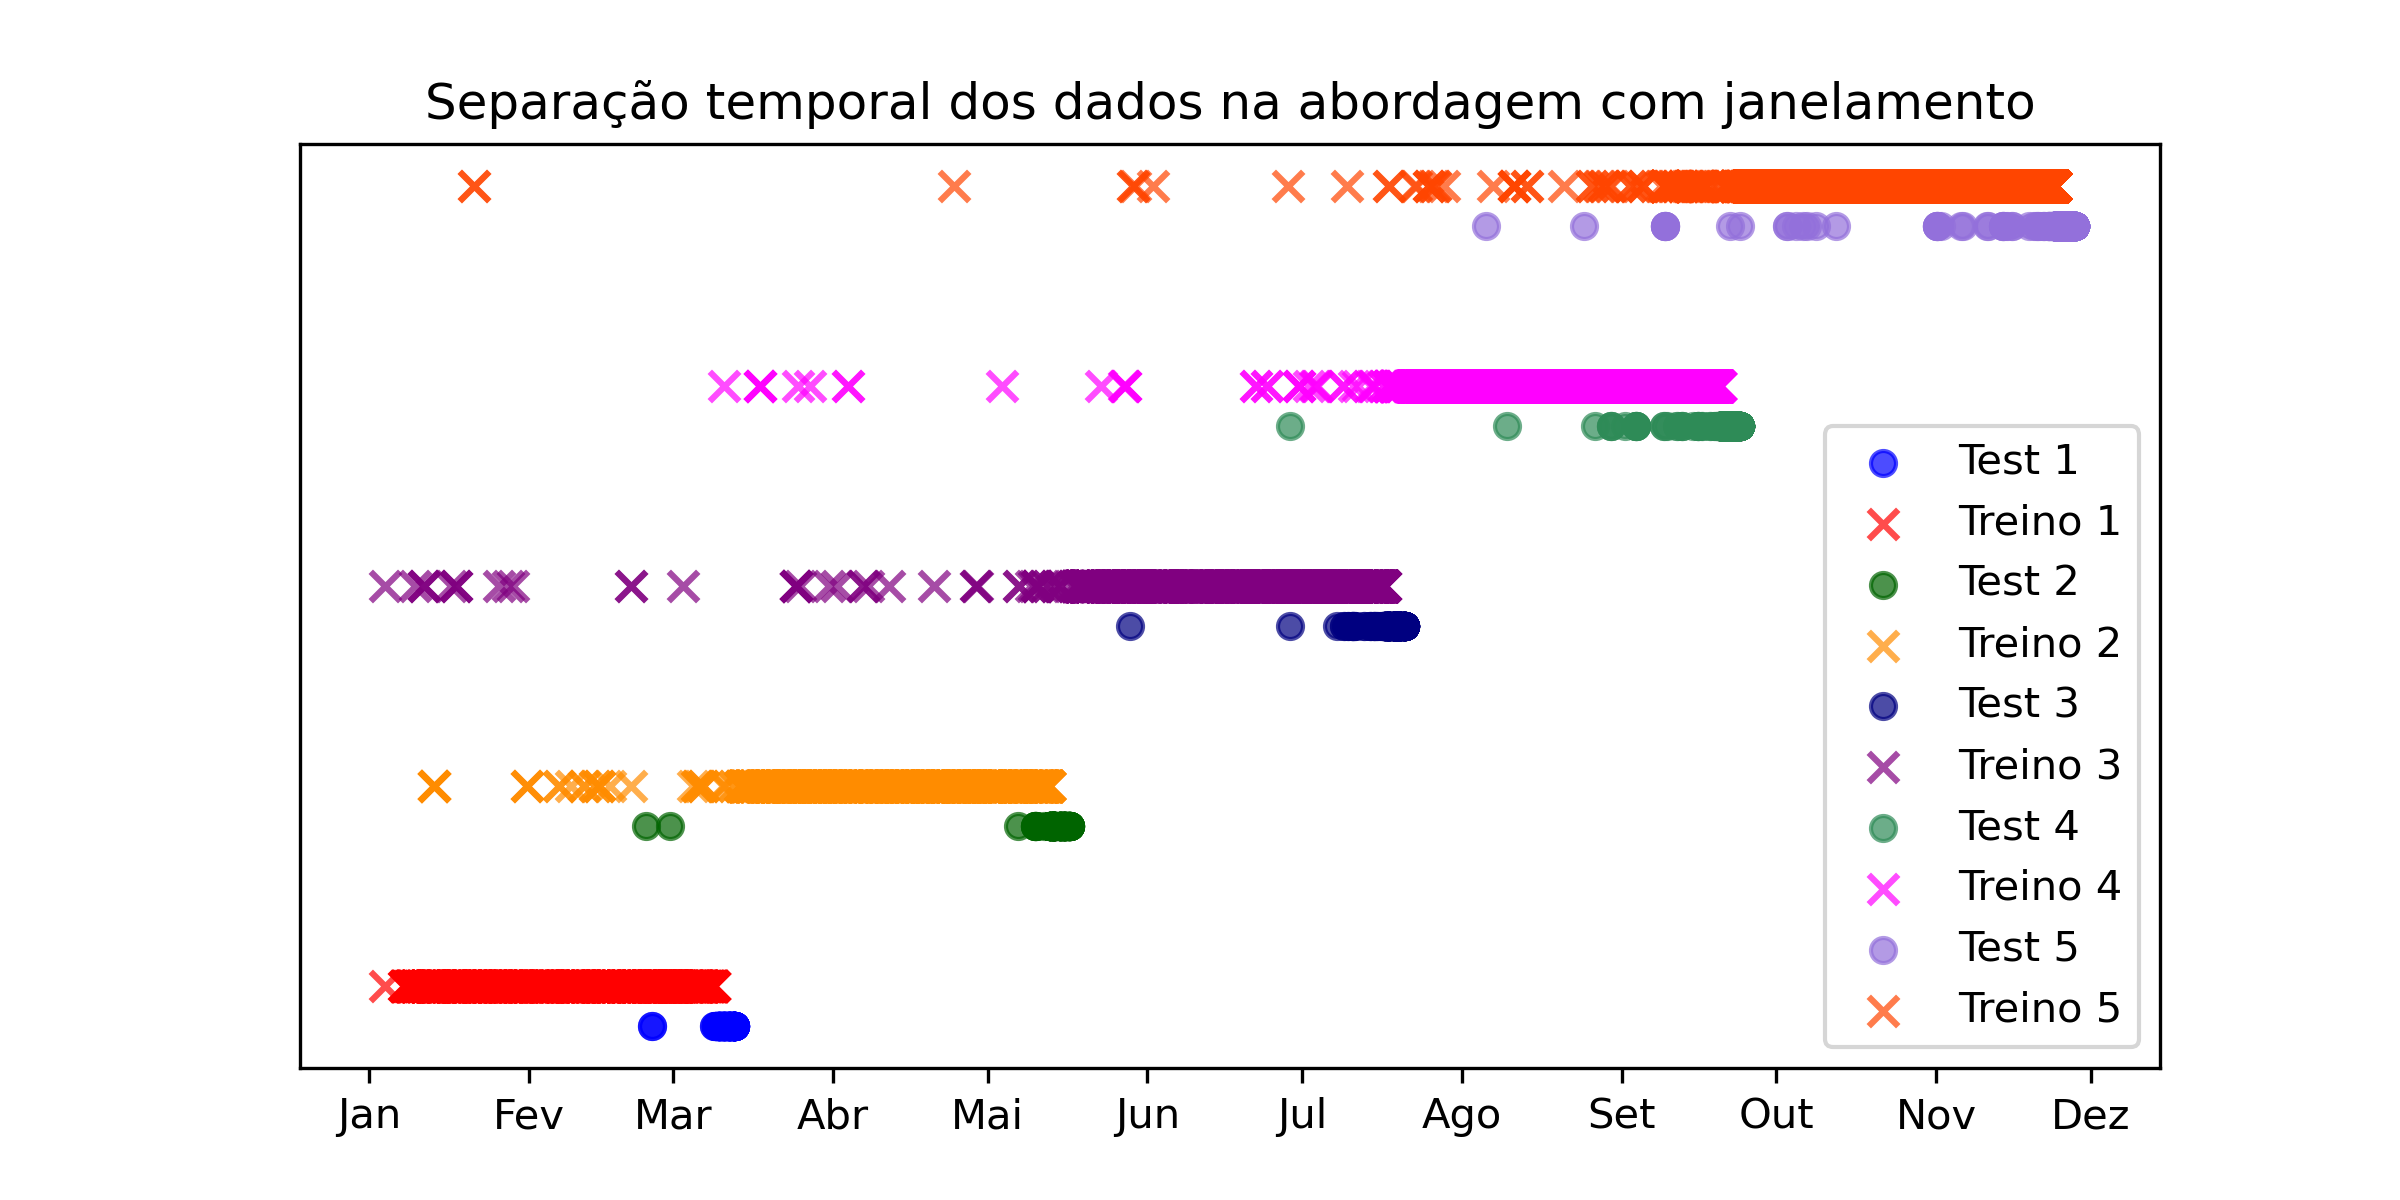
\includegraphics[width=0.8\textwidth]{chapters/chap04/images/scatter_plot.png}
  \caption{Distribuição das sessões por janela de tempo na abordagem
  \textit{windowed}, ao longo do ano de 2023.}
  \label{fig:scatter_plot}
\end{figure}


  \begin{table}
    \centering
    \begin{tabular}{|l|l|l|l|l|l|l|}
      \hline
      Conjunto & Eventos & Sessões & Itens & $\Delta$ & $\sigma$ & Janela de tempo \\ \hline 
         Treinamento & 90.801 & 26.649 & 1.702 & 3,3 & 2,0 & 01/01/2023 a 03/12/2023 \\ \hline
        Teste & 11.265 & 3.106 & 589 & 3,6 & 2,0 & 02/08/2023 a 18/12/2023 \\ \hline
    \end{tabular}
    \caption{Informações sobre o \textit{dataset} utilizado na abordagem
    \textit{single}. $\Delta$ e $\sigma$ são a média e o desvio padrão da quantidade de
    usuários por sessão.}
    \label{tab:split_data}
  \end{table}

  \begin{figure}[ht]
    \centering
    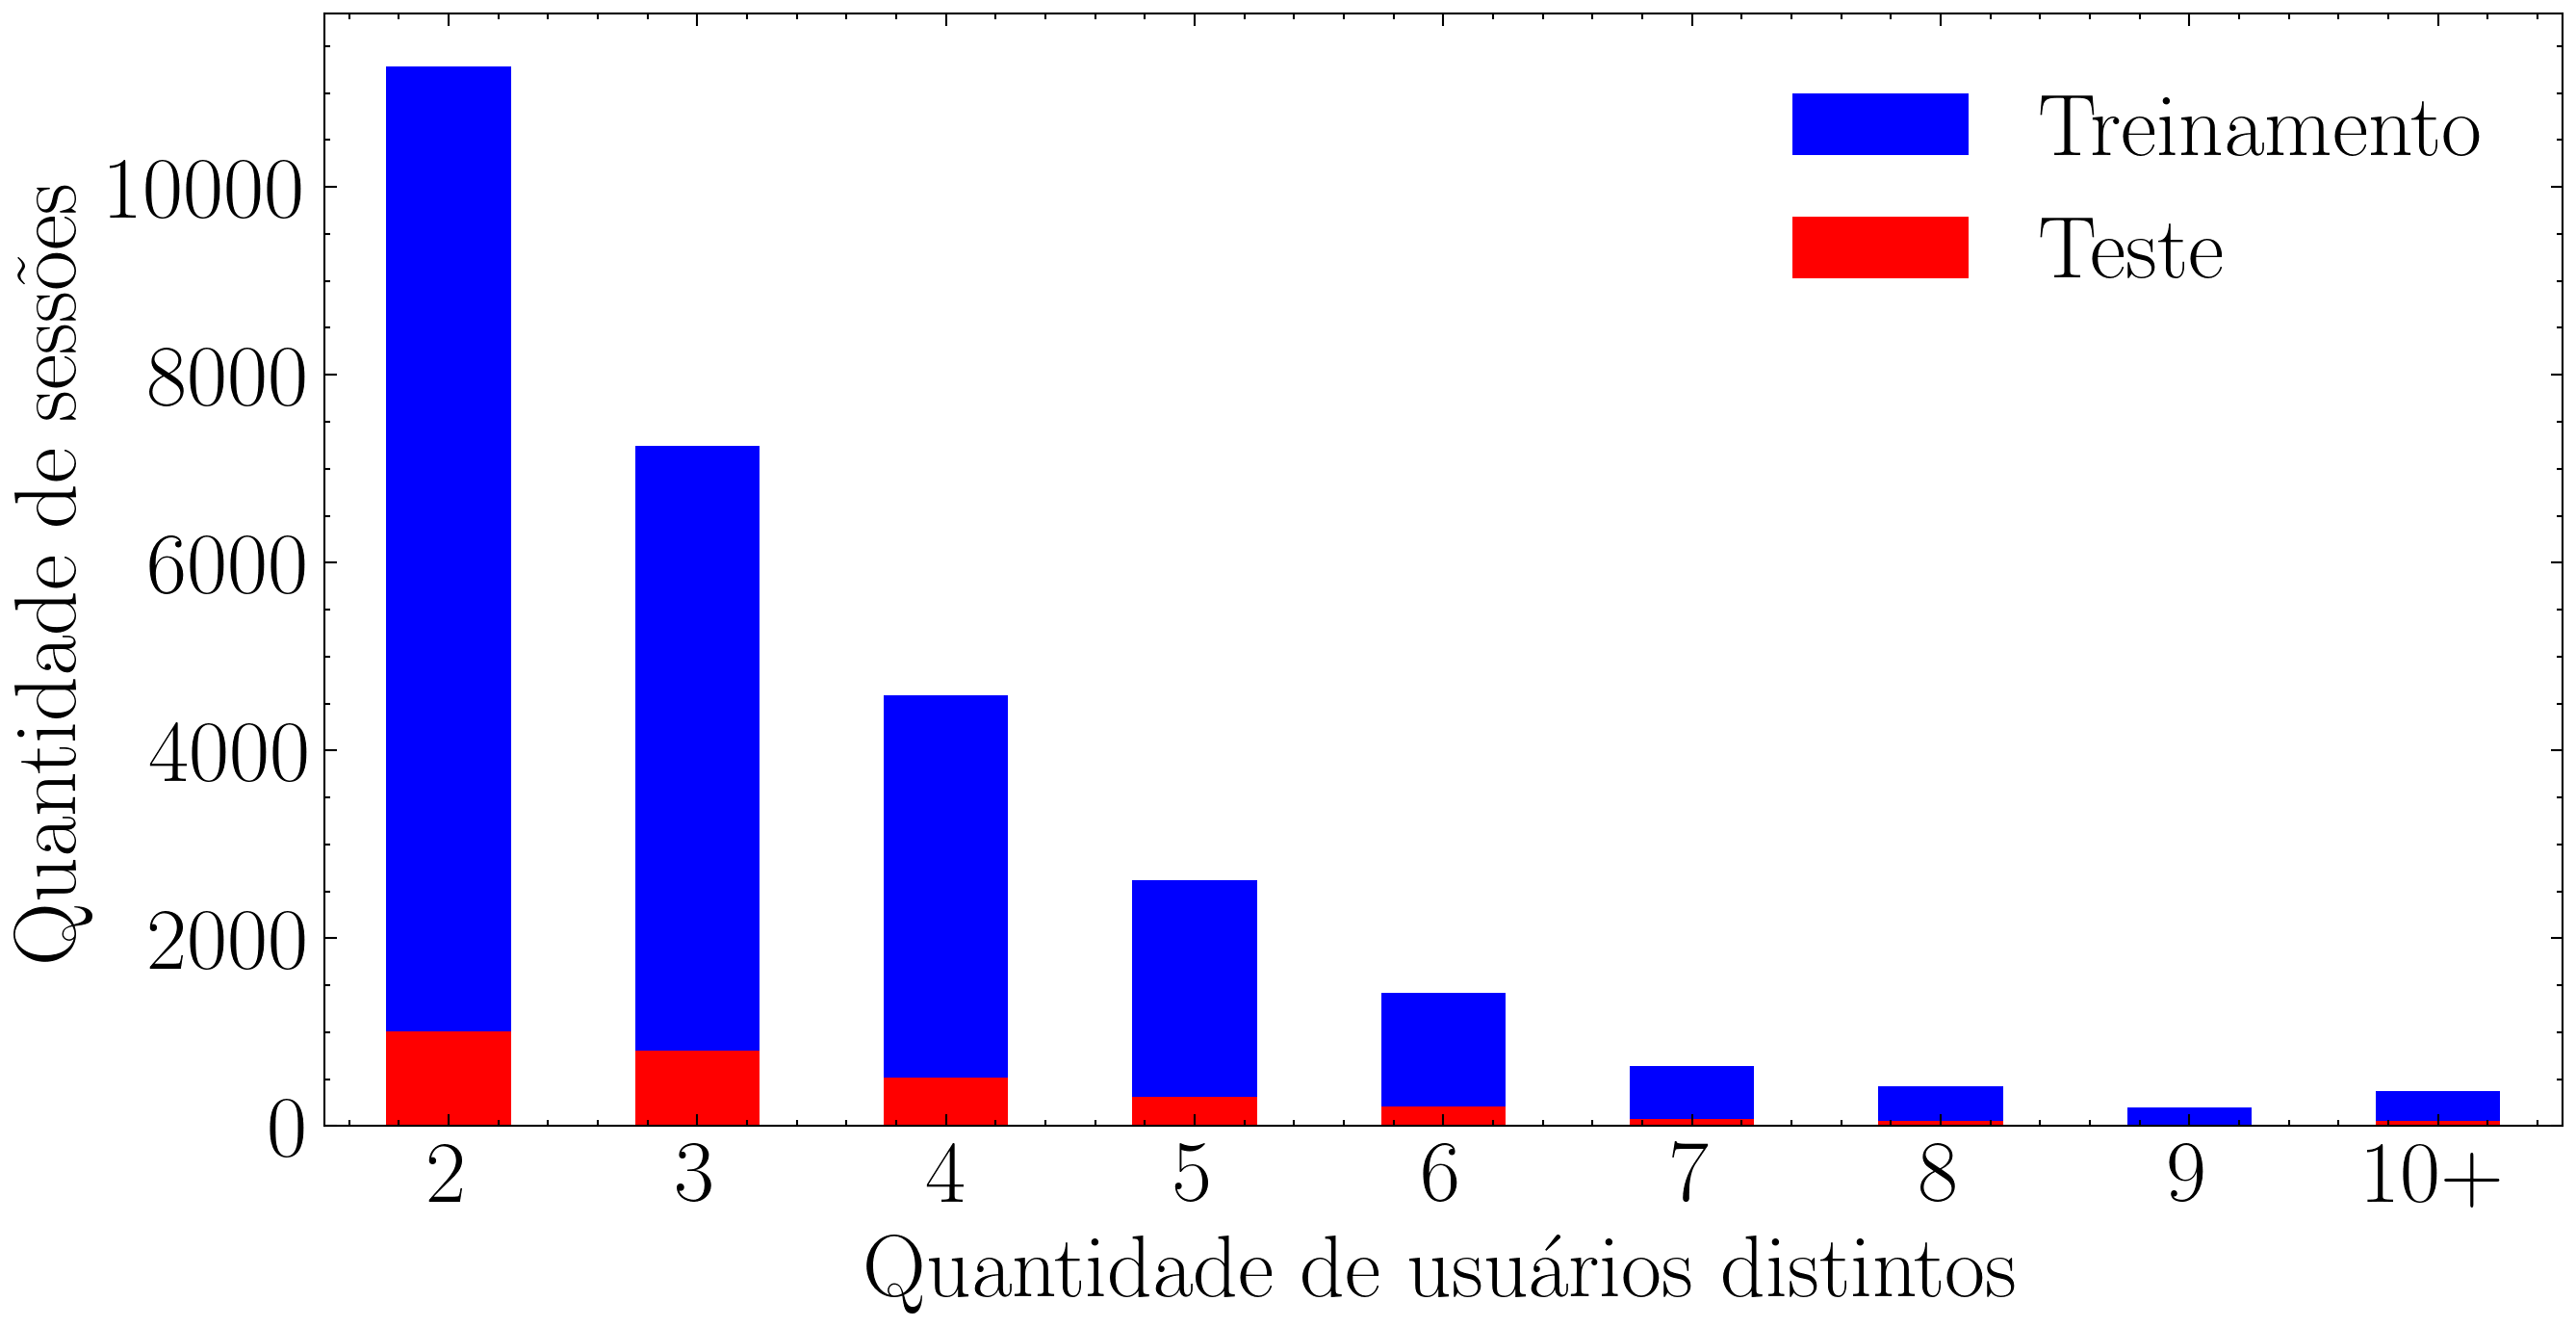
\includegraphics[width=0.8\textwidth]{chapters/chap04/images/histograma.png}
    \caption{Distribuição da quantidade de usuários por sessão na abordagem
    \textit{single}. A distribuição de treinamento está empilhada acima da
    distribuição de teste.}
    \label{fig:next-item-single}
  \end{figure}

% Na abordagem apresentada, apenas a primeira interação de cada usuário na
% sessão consta na base, de forma que nenhum usuário apareça mais de uma vez na
% mesma sessão. Dessa forma, a tarefa do modelo é prever qual será o próximo usuário
% inédito a contribuir na sessão.


  % build a table with 5 experiments. columns are if is session-based or aware, single-split or windowed, and the evaluation method.

  \chapter{Resultados}
  % \section{Experimentos} 

% \begin{table}[htbp]
%   \centering
%   \begin{tabular}{|l|l|l|l|}
%     \hline
%       & Eventos & Sessões & Itens \\ \hline
%      \textit{Dataset} completo & 154.121 & 77.055 & 20.840 \\ \hline
%       \textit{Dataset} filtrado & 105.955 & 31.103 & 2.579 \\ \hline
%       Conjunto completo de treinamento & 99.714 & 29.328 & 2.452 \\ \hline
%       conjunto de teste & 5.516 & 1.530 & 477 \\ \hline
%       Conjunto de treinamento & 93.679 & 27.605 & 2.320 \\ \hline
%       Conjunto de validação & 5.291 & 1.467 & 475 \\ \hline
%       Conjunto de otimização & 304 & 100 & 111 \\ \hline
%   \end{tabular}
%   \caption{Informações sobre o \textit{dataset} utilizado na abordagem \textit{single}.}
%   \label{tab_dataset}
% \end{table}

\section{Abordagem \textit{single-split}, \textit{session-based}, \textit{next-item}}




 

  \subsubsection{Modelos não-personalizados}

  Pop é o modelo de popularidade, com pontuações proporcionais ao suporte dos
  itens, limitado aos 100 itens mais populares. Random é o modelo aleatório,
  retornando uma pontuação aleatória para cada item. SPop é o modelo de
  popularidade de sessão, em que as pontuações são proporcionais à maior
  frequência dos itens em cada sessão, também limitado aos 100 itens mais
  populares. Finalmente, RPop é o modelo de popularidade para sessões recentes,
  em que apenas itens do último dia são considerados por padrão. Foi utilizada a
  avaliação sobre o próximo item da sessão.
\begin{table}[htbp]
  \centering
  \begin{tabular}
    {|l|l|l|l|l|l|l|l|l|}
    \hline
    Modelo & HR@5 & HR@10 & MRR@5 & MRR@10 & NDCG@10 & Cov@10 & Pop@10 \\ \hline
    Pop & 0,132 & 0,268 & 0,092 & 0,110 & 0,155 & 0,006 & 0,531 \\ \hline
    Random & 0,003 & 0,006 & 0,001 & 0,002 & 0,003 & \textbf{1,000} & \textbf{0,013} \\ \hline
    RPop & \textbf{0,204} & \textbf{0,294} & \textbf{0,125} & \textbf{0,137} & \textbf{0,204} & 0,010 & 0,321 \\ \hline
    SPop & 0,109 & 0,221 & 0,045 & 0,058 & 0,114 & 0,301 & 0,473 \\ \hline
  \end{tabular}
\end{table}

De forma esperada, o modelo Random maximiza a cobertura, minimizando o índice de
popularidade. O modelo de popularidade para sessões recentes (RPop) apresenta
resultados superiores aos demais modelos de popularidade.
Em seguida, na tabela \ref{tab_baseline}, são apresentados os resultados para os
modelos de mineração de padrões e vizinhança, fatoração de matrizes e redes neurais.


\subsubsection{Modelos por mineração de padrões e vizinhança}

\begin{table}[htbp]
  \abbrev{CT}{\textit{Context Tree}}
  \abbrev{AR}{Regras de associação}
  \abbrev{SR}{Regras de sequência}
  \centering
  \begin{tabular}{|l|l|l|l|l|l|l|r|}
    \hline
    Modelo & HR@5 & HR@10 & MRR@5 & MRR@10 & Cov@10 & Pop@10 & $\Delta t_{treino} [s]$ \\
    \hline
    CT & \textbf{0,541} & \textbf{0,631} & \textbf{0,392} & \textbf{0,404} & 0,518 & 0,358 & 8,3 \\
    \hline        
    $\text{SR}_{2}$ & 0,468 & 0,593 & 0,292 & \textbf{0,310} & 0,507 & 0,260 & 0,1 \\
    \hline
    Markov  & 0,465 & 0,583 & 0,292 & 0,308 & 0,488 & 0,247 & 0,1 \\
    \hline
    $\text{SR}_{1}$ & 0,461 & 0,583 & 0,291 & 0,308 & 0,492 & 0,272 & 0,1 \\
    \hline
    $\text{skNN}_{2}$ & 0,444 & 0,604 & 0,157 & 0,179 & 0,603 & 0,217 & 0,1 \\
    \hline
    $\text{VSTAN}_{1}$ & 0,419 & 0,573 & 0,161 & 0,182 & 0,553 & 0,230 & 0,1 \\
    \hline
    $\text{VSTAN}_{2}$ & 0,412 & 0,582 & 0,148 & 0,171 & 0,571 & 0,236 & 0,1 \\
    \hline
    $\text{skNN}_{1}$ & 0,406 & 0,564 & 0,151 & 0,172 & \textbf{0,636} & \textbf{0,187} & 0,1 \\
    \hline
    AR & 0,403 & 0,531 & 0,238 & 0,255 & 0,488 & 0,284 & 0.1 \\
    \hline
    $\text{STAN}_{1}$ & 0,403 & 0,570 & 0,147 & 0,170 & 0,516 & 0,271 & 0.1 \\
    \hline
    $\text{STAN}_{2}$ & 0,366 & 0,551 & 0,126 & 0,151 & 0,562 & 0,196 & 0.1 \\
    \hline
$\text{vsKNN}_{1}$ & 0,365 & 0,527 & 0,136 & 0,158 & 0,312 & 0,222 & 0.1 \\
\hline
\hline
    $\text{smf}_1$ & \textbf{0,521} & \textbf{0,637} & \textbf{0,339} & \textbf{0,354} & 0,613 & 0,228 & 1146,6 \\
    \hline
    $\text{smf}_2$ & 0,506 & 0,616 & 0,332 & 0,346 & 0,321 & 0,256 & 987,4 \\
    \hline
    FPMC & 0,289 & 0,421 & 0,122 & 0,140 & 0,840 & \textbf{0,226} & 921,7 \\
    \hline
    FISM & 0,280 & 0,414 & 0,126 & 0,144 & 0,824 & 0,264 & 918,7 \\
    \hline
    BPRMF & 0,253 & 0,397 & 0,107 & 0,125 & 0,834 & 0,233 & 918,3 \\
    \hline
    Fossil & 0,243 & 0,399 & 0,100 & 0,121 & \textbf{0,848} & 0,253 & 917,7 \\
    \hline
    \hline
    $\text{GNN}_1$ & \textbf{0,594} & \textbf{0,666} & \textbf{0,439} & \textbf{0,450} & 0,749 & 0,221 & 483,7 \\
    \hline
    $\text{GNN}_2$ & 0,588 & \textbf{0,666} & 0,425 & 0,435 & 0,713 & 0,220 & 464,6 \\
    \hline
    $\text{STAMP}_1$ & 0,543 & 0,639 & 0,385 & 0,398 & 0,672 & 0,244 & 106,6 \\
    \hline
    $\text{STAMP}_2$ & 0,539 & 0,638 & 0,384 & 0,397 & 0,635 & 0,243 & 106,6 \\
    \hline  
    $\text{NextItNet}_1$ & 0,426 & 0,526 & 0,277 & 0,290 & 0,336 & 0,278 & 1205,7 \\
    \hline
    $\text{NextItNet}_2$ & 0,410 & 0,518 & 0,278 & 0,293 & 0,312 & 0,287 & 966,4 \\
    \hline
    $\text{NARM}_1$ & 0,293 & 0,394 & 0,173 & 0,186 & \textbf{0,718} & 0,220 & 6633,7 \\
    \hline
    $\text{NARM}_2$ &  0,273 & 0,377 & 0,165 & 0,179 & 0,699 & \textbf{0,213} & 2598,8 \\
    \hline
    $\text{GRU4Rec}$ & 0,262 & 0,371 & 0,144 & 0,145 & 0,643 & 0,205 & 542,3 \\
    \hline
    $\text{CSRM}_1$ & 0.229 & 0.315 & 0.134 & 0.146 & 0.623 & 0.148 &  128,5 \\
    \hline
    $\text{CSRM}_2$ & 0.237 & 0.328 & 0.143 & 0.155 & 0.640 & 0.158 & 127,4 \\
    \hline
  
%     Metrics;HitRate@5: ;HitRate@10: ;MRR@5: ;MRR@10: ;Coverage@10: ;Popularity@10: ;
% ct;0.5418556195612207;0.6307145483515136;0.3915941496098388;0.4036660752465399;0.517626321974148;0.3575665829610209;
      \end{tabular}
  \caption{Resultado para os modelos avaliando o próximo item da sessão, agrupados por
  abordagem: mineração de padrões e vizinhança, fatoração e redes neurais.
  Os hiperparâmetros utilizados para cada modelo estão descritos no apêndice.}
  %  $\text{SR}_{1}$
  % e $\text{SR}_{2}$ são os modelos de regras de sequência com 6 e 11 passos, com peso inverso e quadrático.
  % $\text{skNN}_{1}$ e $\text{skNN}_{2}$ são os modelos de kNN com 50 e 100 vizinhos, ambos com função de similaridade cosseno.
  % $\text{vsKNN}_{1}$ e $\text{vsKNN}_{2}$ são os modelos de kNN com 1500 e 50 vizinhos, com amostragem de 10.000 e 2.500, respectivamente, ambos com função de similaridade cosseno.
  % vstan-k=1000-sample_size=5000-similarity=cosine-lambda_spw=10-lambda_snh=40-lambda_inh=5-lambda_ipw=1e-05-lambda_idf=False
  % vstan-k=2000-sample_size=1000-similarity=vec-lambda_spw=10-lambda_snh=100-lambda_inh=0.625-lambda_ipw=0.125-lambda_idf=False
  % $stan_{1}$ e $stan_{2}$ são os modelos de kNN com 1000 e 2000 vizinhos, com
  % amostragem de 5000 e 1000, respectivamente, com função de similaridade
  % cosseno e vetorial,   
  \label{tab_baseline}  
\end{table}

Inclui regras de associação, cadeias de Markov, regras de
sequência. Também é realizada para métodos de vizinhança: kNN, vskNN, STAN e
VSTAN. Os modelos SR, skNN e vsKNN são otimizados com seus respectivos
hiperparâmetros, obtidos a partir de uma otimização do MRR@10.

Os modelos de regras de sequência e baseados em cadeias de Markov, inclusive a
árvore de contexto, apresentam resultados superiores, considerando as métricas
HR@5, HR@10 e MRR@5 e MRR@10. Apesar dos modelos de vizinhança apresentarem
bons resultados para o HR, o MRR decai consideravelmente nesses modelos.

Quando comparados aos demais agrupamentos, os modelos por mineração de padrões e
vizinhança obtiveram bons resultados para HR@5 e HR@10. Entre os modelos de
vizinhança, o modelo $\text{skNN}_2$ apresentou os melhores resultados, seguido pelo
modelo $\text{VSTAN}_1$, que é modelo mais complexo dentre os modelos de vizinhança.

\subsubsection{Métodos baseados em fatoração}
Avalia-se os modelos FPMC, FISM, Fossil,
BPRMF e smf. Os modelos smf apresentam resultados bem superiores aos demais, tanto no HitRate
quanto no MRR. Vale observar que a duração do treinamento de cada um dos modelos
baseados em fatoração é consideravelmente maior do que os modelos de mineração
de padrões e vizinhança.

\subsubsection{Modelos baseados em redes neurais}
Inclui os modelos GRU4Rec, NARM, NextItNet, STAMP, GNN e CSRM. Os modelos GNN e
STAMP apresentam os melhores resultados globais para as medidas de HR. Os
modelos STAMP e NextItNet apresentam bons resultados, enquanto que os modelos
NARM, GRU4Rec e CSRM apresentam resultados inferiores, inclusive quando comparados
a modelos mais simples, tais como regras de sequência ou baseados em vizinhança.


\section{Abordagem \textit{windowed}, \textit{session-based}, \textit{next-item}}
\begin{table}[htbp]
  \centering
  \begin{tabular}{|c|c|c|c|c|c|}
    \hline
    Conjunto & Índice & Eventos & Sessões & Itens & Data\\
    \hline
    Treinamento & 1 & 3190 & 1098 & 145 & 08/01/2023 a 09/03/2023\\
    \hline
    Teste & 1 & 205 & 72 & 40 & 09/03/2023 a 13/03/2023\\
    \hline
    Treinamento & 2 & 3976 & 1346 & 197 & 14/03/2023 a 13/05/2023\\
    \hline
    Teste & 2 & 244 & 68 & 53 & 13/05/2023 a 17/05/2023\\
    \hline
    Treinamento & 3 & 7407 & 2191 & 301 & 18/05/2023 a 17/07/2023\\
    \hline
    Teste & 3 & 466 & 162 & 100 & 17/07/2023 a 21/07/2023\\
    \hline
    Treinamento & 4 & 21683 & 6267 & 754 & 22/07/2023 a 20/09/2023\\
    \hline
    Teste & 4 & 1779 & 454 & 201 & 20/09/2023 a 24/09/2023\\
    \hline
    Treinamento & 5 & 43993 & 12852 & 1681 & 25/09/2023 a 24/11/2023\\
    \hline
    Teste & 5 & 2978 & 830 & 351 & 24/11/2023 a 28/11/2023\\
    \hline
  \end{tabular}
  \caption{Conjuntos de treino e teste separados em cinco janelas para abordagem \textit{windowed}, \textit{session-based}.}
  \label{tab:windowed_data}
\end{table}

Na abordagem
\textit{windowed}, uma janela deslizante é aplicada por todo o período,
separando em cinco pares distintos de treinamento e teste, descritos na tabela
\ref{tab:windowed_data}. Nota-se o aumento gradual da quantidade de eventos,
sessões e itens ao longo do tempo. Os resultados sob abordagem \textit{windowed} são obtidos a partir da média
aritmética dos resultados obtidos em cada janela. Os resultados constam na
tabela \ref{tab:windowed_next_item_all}.


\begin{table}[htbp]
  \centering
  \small
  % reduce space between columns and rows:
  \setlength{\tabcolsep}{2pt}
  \centerline{
  \begin{tabular}{|l|l|l|l|l|l|l|r|}
    \hline
    Modelo & HR@5 & HR@10 & MRR@5 & MRR@10 & Cov@10 & Pop@10 & $\Delta t[s]$ \\
    \hline
    RPop & \textbf{0,222}\textpm0,061 & \textbf{0,356}\textpm0,079 & \textbf{0,116}\textpm0,045 & \textbf{0,13}3\textpm0,046 & 0,065\textpm0,045 & 0,355\textpm0,073 & 0,006 \\
    \hline
    Pop & 0,202\textpm0,056 & 0,325\textpm0,063 & 0,114\textpm0,047 & 0,130\textpm0,045 & 0,034\textpm0,023 & 0,493\textpm0,099 & 0,001 \\
    \hline
      SPop & 0,168\textpm0,073 & 0,298\textpm0,072 & 0,072\textpm0,030 & 0,089\textpm0,029 & 0,235\textpm0,036 & 0,456\textpm0,094 & 0,002 \\
    \hline
    Random & 0,012\textpm0,006 & 0,032\textpm0,019 & 0,007\textpm0,004 & 0,009\textpm0,005 & \textbf{1,000}\textpm0,000 & \textbf{0,045}\textpm0,024 & 0,001 \\
    \hline
    \hline
    $\text{smf}_{1}$ & \textbf{0,401}\textpm0,040 & \textbf{0,532}\textpm0,045 & \textbf{0,247}\textpm0,032 & \textbf{0,264}\textpm0,030 & 0,492\textpm0,020 & \textbf{0,281}\textpm0,082 & 193 \\
    \hline
    $\text{smf}_{2}$ & 0,364\textpm0,030 & 0,495\textpm0,039 & 0,224\textpm0,024 & 0,240\textpm0,024 & 0,271\textpm0,044 & 0,328\textpm0,101 & 162 \\
    \hline
    FISM & 0,291\textpm0,051 & 0,443\textpm0,081 & 0,144\textpm0,038 & 0,164\textpm0,041 & \textbf{0,625}\textpm0,041 & 0,346\textpm0,099 & 892 \\
    \hline
    FPMC & 0,291\textpm0,063 & 0,438\textpm0,088 & 0,140\textpm0,040 & 0,159\textpm0,042 & 0,613\textpm0,041 & 0,350\textpm0,098 & 897 \\
    \hline
    BPRMF & 0,290\textpm0,049 & 0,421\textpm0,054 & 0,149\textpm0,036 & 0,166\textpm0,036 & 0,624\textpm0,044 & 0,343\textpm0,095 & 893 \\
    \hline
    Fossil & 0,288\textpm0,033 & 0,417\textpm0,041 & 0,147\textpm0,028 & 0,164\textpm0,027 & 0,605\textpm0,058 & 0,343\textpm0,091 & 900 \\
    \hline
    \hline
    ct & \textbf{0,413}\textpm0,058 & 0,525\textpm0,053 & \textbf{0{,}274}\textpm0,041 & \textbf{0{,}289}\textpm0,041 & 0,375\textpm0,009 & 0,396\textpm0,098 & 1,198 \\
    \hline
    $\text{SR}_{1}$ & 0,378\textpm0,053 & 0,506\textpm0,054 & 0,225\textpm0,021 & 0,242\textpm0,022 & 0,443\textpm0,055 & 0,281\textpm0,061 & 0,056 \\
    \hline
    $\text{SR}_{2}$ & 0,375\textpm0,058 & 0,508\textpm0,042 & 0,224\textpm0,023 & 0,241\textpm0,023 & 0,453\textpm0,053 & 0,273\textpm0,062 & 0,065 \\
    \hline
    AR & 0,363\textpm0,055 & 0,476\textpm0,041 & 0,207\textpm0,041 & 0,222\textpm0,039 & 0,455\textpm0,067 & 0,300\textpm0,073 & 0,117 \\
    \hline
    $\text{VSTAN}_{1}$ & 0,363\textpm0,048 & 0,505\textpm0,061 & 0,145\textpm0,021 & 0,164\textpm0,022 & 0,487\textpm0,067 & 0,291\textpm0,062 & 0,291 \\
    \hline
      Markov & 0,360\textpm0,054 & 0,477\textpm0,040 & 0,218\textpm0,020 & 0,233\textpm0,020 & 0,438\textpm0,047 & 0,257\textpm0,056 & 0,047 \\
    \hline
      $\text{VSTAN}_{2}$ & 0,358\textpm0,061 & 0,493\textpm0,058 & 0,137\textpm0,024 & 0,155\textpm0,023 & 0,500\textpm0,071 & 0,293\textpm0,063 & 0,293 \\
    \hline
    $\text{skNN}_{1}$ & 0,351\textpm0,075 & \textbf{0,526}\textpm0,061 & 0,140\textpm0,029 & 0,164\textpm0,026 & \textbf{0,534}\textpm0,058 & 0,258\textpm0,062 & 0,079 \\
    \hline
    $STAN_{2}$ & 0,346\textpm0,065 & 0,493\textpm0,057 & 0,129\textpm0,021 & 0,149\textpm0,020 & 0,506\textpm0,071 & 0,262\textpm0,059 & 0,037 \\
    \hline
    $\text{vsKNN}_{2}$ & 0,340\textpm0,051 & 0,477\textpm0,060 & 0,132\textpm0,021 & 0,150\textpm0,018 & \textbf{0,534}\textpm0,056 & \textbf{0,233}\textpm0,052 & 0,077 \\
    \hline
    $STAN_{1}$ & 0,339\textpm0,067 & 0,494\textpm0,072 & 0,132\textpm0,025 & 0,153\textpm0,025 & 0,463\textpm0,071 & 0,324\textpm0,068 & 0,324 \\
    \hline
    $\text{skNN}_{2}$ & 0,334\textpm0,070 & 0,507\textpm0,068 & 0,132\textpm0,024 & 0,156\textpm0,024 & 0,491\textpm0,060 & 0,282\textpm0,065 & 0,021 \\
    \hline
    $\text{vsKNN}_{1}$ & 0,299\textpm0,051 & 0,458\textpm0,040 & 0,119\textpm0,020 & 0,140\textpm0,019 & 0,511\textpm0,075 & 0,267\textpm0,060 & 0,029 \\
    \hline
    \hline
    $\text{GNN}_2$ & \textbf{0{,}421}\textpm0,049 & \textbf{0{,}551}\textpm0,056 & \textbf{0,264}\textpm0,062 & \textbf{0,280}\textpm0,061 & 0,517\textpm0,055 & 0,296\textpm0,089 & 122 \\
    \hline
    $\text{STAMP}_2$ & 0,395\textpm0,039 & 0,515\textpm0,035 & 0,249\textpm0,037 & 0,266\textpm0,035 & 0,592\textpm0,041 & 0,268\textpm0,071 & 31,1 \\
    \hline
    $\text{GNN}_1$ & 0,393\textpm0,062 & 0,496\textpm0,068 & 0,254\textpm0,056 & 0,268\textpm0,056 & 0,544\textpm0,060 & 0,291\textpm0,079 & 120 \\
    \hline
    $\text{STAMP}_1$ & 0,382\textpm0,047 & 0,501\textpm0,042 & 0,253\textpm0,047 & 0,269\textpm0,046 & 0,599\textpm0,059 & 0,269\textpm0,059 & 32,0 \\
    \hline
    $\text{NextItNet}_2$ & 0,352\textpm0,045 & 0,461\textpm0,039 & 0,235\textpm0,042 & 0,250\textpm0,041 & 0,381\textpm0,088 & 0,316\textpm0,097 & 83,8 \\  
    \hline
    $\text{NextItNet}_1$ & 0,336\textpm0,076 & 0,451\textpm0,059 & 0,221\textpm0,059 & 0,236\textpm0,056 & 0,326\textpm0,107 & 0,327\textpm0,109 & 107,3 \\
    \hline
    $\text{NARM}_2$ & 0,295\textpm0,048 & 0,426\textpm0,067 & 0,173\textpm0,034 & 0,190\textpm0,037 & 0,586\textpm0,049 & 0,264\textpm0,076 & 193,9 \\
    \hline
    $\text{NARM}_1$ & 0,274\textpm0,037 & 0,418\textpm0,059 & 0,167\textpm0,024 & 0,187\textpm0,026 & 0,576\textpm0,029 & 0,267\textpm0,085 & 372,2 \\
    \hline
    $\text{CSRM}_1$ & 0,201\textpm0,034 & 0,300\textpm0,030 & 0,117\textpm0,017 & 0,130\textpm0,016 & 0,492\textpm0,063 & 0,267\textpm0,085 & 19,8 \\
    \hline
    $\text{CSRM}_2$ & 0,191\textpm0,029 & 0,306\textpm0,050 & 0,104\textpm0,027 & 0,119\textpm0,028 & 0,439\textpm0,046 & 0,278\textpm0,085 & 19,9 \\
    \hline
    GRU4Rec & 0,176\textpm0,055 & 0,235\textpm0,073 & 0,099\textpm0,016 & 0,107\textpm0,018 & \textbf{0,731}\textpm0,088 & \textbf{0,079}\textpm0,051 & 63,3 \\
    \hline
    \end{tabular}
  } \caption{Resultado dos modelos \textit{session-based} na abordagem
  \textit{windowed}, avaliando o próximo item da sessão. Valores exibidos são a
  média dos cinco \textit{splits} acompanhada da variância. Valores agrupados por abordagem e ordenados
  internamente por HR@5. Maiores valores para cada medida de desempenho
  estão em negrito nos agrupamentos.}
\label{tab:windowed_next_item_all}
\end{table}


Para cada agrupamento de modelos, os modelos smf, ct, SR, GNN e STAMP novamente
apresentam os melhores resultados, tal que a GNN novamente apresenta o melhor
resultado global para as métricas HR@5, HR@10. Novamente,
 os modelos CSRM e GRU4Rec apresentam os piores resultados globais para o
HR@5 e HR@10.

Na figura
\ref{fig:next-item-single-123}, é possível observar que os modelos de redes neurais
começam com resultados inferiores aos demais modelos, mas passam a superar os
demais conforme a quantidade de eventos por \textit{split} aumenta. Essa
observação condiz com a característica de modelos de aprendizado profundo, em
geral, dependerem de uma grande quantidade de dados para apresentarem resultados
superiores. A figura \ref{fig:progressao} apresenta a progressão do HR e MRR conforme a
quantidade de valores preditos para cada métrica.


\begin{figure}[htbp]
  \centering
  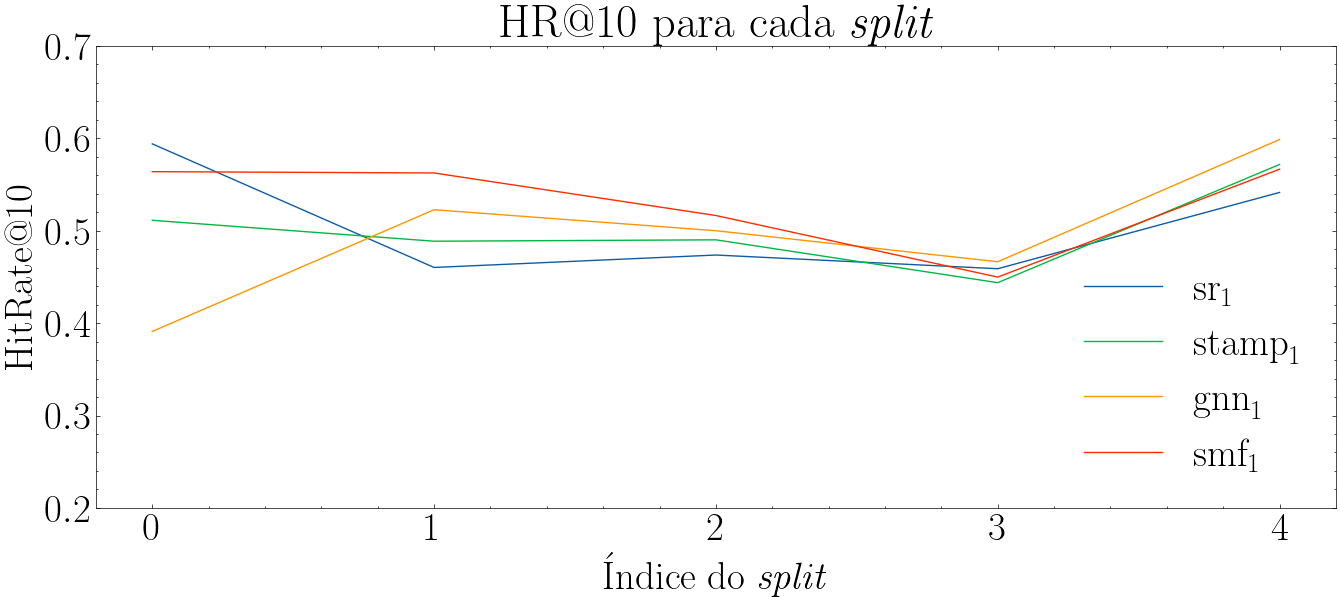
\includegraphics[width=1\textwidth]{chapters/chap04/images/hr10_splits.png}
  \caption{HR@10 em cada janela para alguns modelos da tabela
  \ref{tab:windowed_next_item_all}.}
  \label{fig:next-item-single-123}
\end{figure}


\begin{figure}[htbp]
  \hfill
  \subfigure{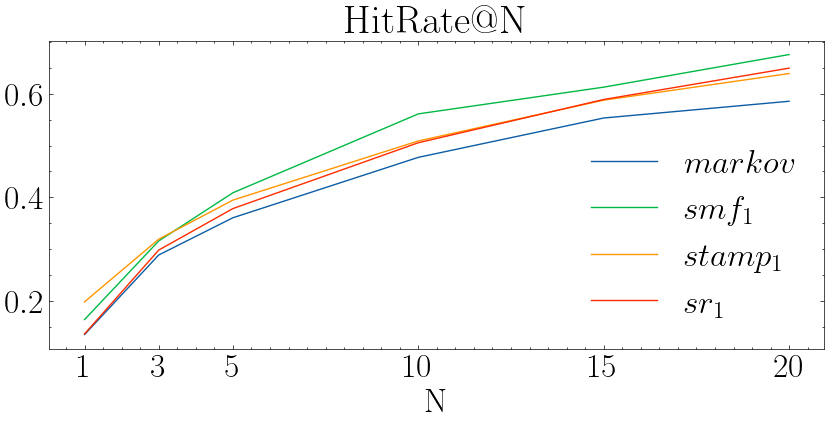
\includegraphics[width=7cm]{chapters/chap04/images/pplotHitRate_n.png}}
  \hfill
  \subfigure{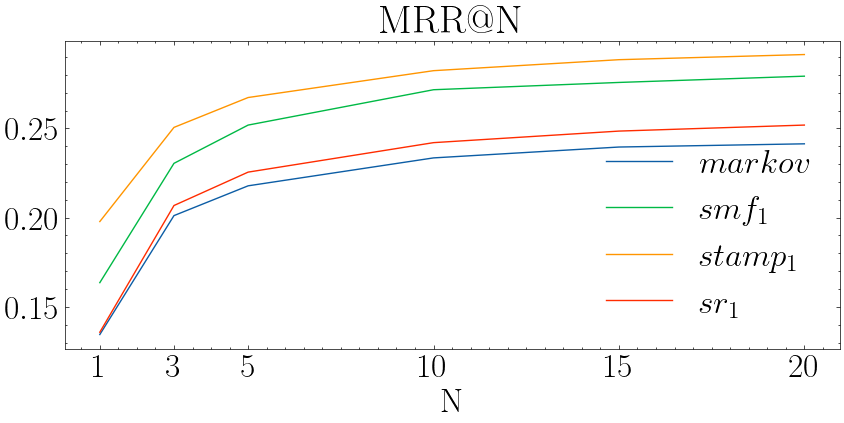
\includegraphics[width=7cm]{chapters/chap04/images/pplotMRR_n.png}}
  \hfill
  \caption{Progressão do HR e MRR conforme a quantidade de valores preditos.}
  \label{fig:progressao}
  \end{figure}

\section{Abordagem \textit{windowed}, \textit{session-based}, \textit{remaining-items}}
Para a abordagem \textit{remaining-items}, foi realizada uma nova otimização
considerando a métrica MAP@10, uma vez que essa métrica substitui o HR@10 para
avaliações de listas ou de conjuntos de itens. Dessa forma, os modelos com nome subscrito aqui presentes possuem hiperparâmetros
distintos da abordagem anterior, constando no apêndice.

Os modelos que apresentaram melhores resultados para precisão, \textit{recall},
NDCG e MAP foram os mesmos dos experimentos anteriores: smf, ct, SR, GNN e
STAMP. Uma diferença observada foi o pior inferior do modelo baseado em cadeia
de Markov de primeira ordem dentro de seu agrupamento, apesar do modelo de árvore de contexto permenecer
com bons resultados. Também é possível observar que os modelos do agrupamento
de regras de sequência e baseados em vizinhança obtiveram bons resultados, quando
comparados aos demais agrupamentos.


\begin{table}
  \centering
  \small
  \centerline{
  \begin{tabular}{|l|l|l|l|l|l|l|}
    \hline
    Modelos & P@10 & R@10 & NDCG@10 & MAP@10 & Cov@10 & Pop@10 \\
    \hline
    rpop & $\mathbf{0{,}086}$\textpm0{,}011 & $\mathbf{0{,}361}$\textpm0{,}092 & \textbf{0{,}240}\textpm0{,}060 & $\mathbf{0{,}042}$\textpm0{,}011 & 0{,}065\textpm0{,}045 & 0{,}355\textpm0{,}073 \\
    \hline
    pop & 0,075\textpm0,025 & 0,326\textpm0,063 & 0,220\textpm0,047 & 0,038\textpm0,010 & 0,034\textpm0,023 & 0,493\textpm0,099 \\
    \hline
    spop & 0,065\textpm0,017 & 0,298\textpm0,053 & 0,179\textpm0,036 & 0,032\textpm0,009 & 0,235\textpm0,036 & 0,456\textpm0,094 \\
    \hline
    random & 0,007\textpm0,004 & 0,033\textpm0,023 & 0,018\textpm0,011 & 0,003\textpm0,002 & \textbf{1,000}\textpm0,000 & \textbf{0,046}\textpm0,024 \\
    \hline
    \hline
    $\text{smf}_2$ & \textbf{0,100}\textpm0,017 & \textbf{0,459}\textpm0,035 & \textbf{0,338}\textpm0,027 & \textbf{0,055}\textpm0,006 & 0,343\textpm0,044 & \textbf{0,321}\textpm0,103 \\
    \hline
    $\text{smf}_1$ & \textbf{0,100}\textpm0,017 & 0,450\textpm0,035 & 0,333\textpm0,023 & \textbf{0,055}\textpm0,005 & 0,242\textpm0,043 & 0,347\textpm0,109 \\
    \hline
    fpmc & 0,086\textpm0,014 & 0,403\textpm0,079 & 0,267\textpm0,049 & 0,044\textpm0,007 & 0,607\textpm0,069 & 0,345\textpm0,094 \\
    \hline
    bprmf & 0,084\textpm0,013 & 0,389\textpm0,066 & 0,260\textpm0,049 & 0,044\textpm0,007 & 0,612\textpm0,051 & 0,347\textpm0,093 \\
    \hline
    fism & 0,083\textpm0,011 & 0,396\textpm0,084 & 0,264\textpm0,055 & 0,045\textpm0,009 & \textbf{0{,}616}\textpm0,047 & 0,346\textpm0,101 \\
    \hline
    fossil & 0,081\textpm0,014 & 0,373\textpm0,048 & 0,252\textpm0,042 & 0,042\textpm0,005 & 0,606\textpm0,042 & 0,346\textpm0,093 \\
    \hline
    \hline
    $\text{SR}_1$ & \textbf{0,104}\textpm0,018 & 0,457\textpm0,055 & 0,337\textpm0,030 & 0,057\textpm0,007 & 0,434\textpm0,061 & 0,286\textpm0,066 \\
    \hline
    ct & 0,103\textpm0,015 & 0,479\textpm0,047 & \textbf{0,367}\textpm0,039 & 0,056\textpm0,006 & 0,375\textpm0,009 & 0,396\textpm0,098 \\
    \hline
     $\text{vsknn}_1$ & $0{,}101$\textpm0,015 & 0,471\textpm0,054 & 0,301\textpm0,036 & 0,057\textpm0,008 & 0,477\textpm0,063 & 0,295\textpm0,067 \\
    \hline
   $\text{SR}_2$ & 0,101\textpm0,014 & 0,455\textpm0,051 & 0,332\textpm0,035 & 0,056\textpm0,006 & 0,453\textpm0,053 & 0,273\textpm0,062 \\
    \hline
     $\text{STAN}_1$ & 0,100\textpm0,011 & $\mathbf{0{,}482}$\textpm0,068 & $0{,}303$\textpm0,042 & $\mathbf{0{,}059}$\textpm0,008 & 0,464\textpm0,067 & 0,304\textpm0,064 \\
    \hline
    $\text{STAN}_2$ & 0,099\textpm0,012 & 0,469\textpm0,072 & 0,296\textpm0,043 & 0,057\textpm0,008 & 0,467\textpm0,071 & 0,316\textpm0,065 \\
    \hline
    ar & 0,098\textpm0,014 & 0,442\textpm0,047 & 0,331\textpm0,040 & 0,054\textpm0,006 & 0,455\textpm0,067 & 0,300\textpm0,073 \\
   \hline
    $\text{VSTAN}_1$ & 0,098\textpm0,013 & 0,463\textpm0,070 & 0,296\textpm0,047 & 0,057\textpm0,008 & 0,468\textpm0,072 & 0,319\textpm0,068 \\
    \hline
    $\text{skNN}_1$ & 0,097\textpm0,012 & 0,471\textpm0,072 & 0,294\textpm0,042 & 0,056\textpm0,009 & 0,468\textpm0,068 & 0,318\textpm0,075 \\
    \hline
    $\text{skNN}_2$ & 0,095\textpm0.014 & 0,487\textpm0,065 & 0,300\textpm0,045 & 0,057\textpm0,009 & 0,540\textpm0,055 & 0,260\textpm0,059 \\
    \hline
    $\text{vsKNN}_2$ & 0,091\textpm0,019 & 0,426\textpm0,051 & 0,268\textpm0,033 & 0,051\textpm0,010 & 0,542\textpm0,063 & 0,216\textpm0,047 \\
    \hline
    Markov & 0,091\textpm0,013 & 0,420\textpm0,041 & 0,310\textpm0,031 & 0,050\textpm0,004 & 0,438\textpm0,047 & 0,257\textpm0,056 \\
    \hline
    $\text{vstan}_2$ & 0,088\textpm0,012 & 0,441\textpm0,052 & 0,266\textpm0,033 & 0,052\textpm0,007 & \textbf{0,571}\textpm0,056 & \textbf{0,212}\textpm0,050 \\
   \hline
   \hline
   GNN & \textbf{0,097}\textpm0,020 & \textbf{0,455}\textpm0,056 & \textbf{0,359}\textpm0,044 & \textbf{0,056}\textpm0,009 & 0,603\textpm0,060 & 0,272\textpm0,075 \\
   \hline
   $\text{STAMP}_2$ & \textbf{0,097}\textpm0,018 & 0,453\textpm0,033 & 0,341\textpm0,041 & 0,052\textpm0,006 & 0,608\textpm0,038 & 0,285\textpm0,072 \\
   \hline
   $\text{STAMP}_1$ & 0,096\textpm0,017 & 0,445\textpm0,042 & 0,331\textpm0,043 & 0,052\textpm0,006 & 0,560\textpm0,056 & 0,286\textpm0,080 \\
   \hline
   $\text{NextItNet}_2$ & 0,095\textpm0,014 & 0,435\textpm0,032 & 0,310\textpm0,011 & 0,051\textpm0,003 & 0,531\textpm0,034 & 0,293\textpm0,078 \\
   \hline
   $\text{NextItNet}_1$ & 0,090\textpm0,019 & 0,427\textpm0,036 & 0,314\textpm0,049 & 0,048\textpm0,007 & 0,321\textpm0,115 & 0,340\textpm0,112\\
   \hline
   $\text{NARM}_2$ & 0,079\textpm0,008 & 0,392\textpm0,045& 0,286\textpm0,035 & 0,043\textpm0,004 & 0,641\textpm0,037 & 0,256\textpm0,071 \\
   \hline
   $\text{NARM}_1$ & 0,079\textpm0,010 & 0,381\textpm0,045 & 0,266\textpm0,017 & 0,042\textpm0,004 & 0,610\textpm0,036 & 0,256\textpm0,068 \\
   \hline
  $\text{CSRM}_2$ & 0,067\textpm0,013 & 0,310\textpm0,061 & 0,209\textpm0,043 & 0,034\textpm0,007 & 0,459\textpm0,070 & 0,278\textpm0,099 \\
   \hline
  $\text{CSRM}_1$ & 0,064\textpm0,011 & 0,314\textpm0,054 & 0,210\textpm0,030 & 0,033\textpm0,004 & 0,473\textpm0,052 & 0,279\textpm0,089 \\
   \hline
   $\text{GRU4Rec}_2$ & 0,017\textpm0,015 & 0,081\textpm0,060 & 0,053\textpm0,048 & 0,008\textpm0,007 & 0,416\textpm0,234 & 0,026\textpm0,021 \\
   \hline
   $\text{GRU4Rec}_1$ & 0,008\textpm0,004 & 0,035 \textpm0,015  & 0,022\textpm0,012 & 0,003\textpm0,002 & \textbf{0,707}\textpm0,092 & \textbf{0,022}\textpm0,006 \\
   \hline
  \end{tabular}
  }
  \caption{Resultados para abordagem \textit{remaining-items}. Em ordem, modelos
  de popularidade, fatoração de matrizes, modelos baseados em vizinhança, regras
  de associação e redes neurais.}
  \label{tab:model_metrics}
\end{table}

\newpage

\section{Abordagem \textit{windowed}, \textit{session-aware}, \textit{next-item}}

Em seguida, são apresentados os resultados obtidos com a abordagem
\textit{windowed} e \textit{session-aware}. Os modelos passaram por otimização
de seus hiperparâmetros, cujos resultados constam no apêndice.

A tabela \ref{tab:windowed_data_session_aware} apresenta os conjuntos de treino
e teste separados em cinco janelas. Novamente, é possível observar o aumento
gradual da quantidade de eventos, sessões e itens ao longo dos \textit{splits}.

Metade dos modelos \textit{session-aware} apresentam resultados que superam
todos os modelos da abordagem \textit{session-based}. Os maiores valores para as
medidas de avaliação entre todos os experimentos foram obtidos na presente
abordagem. O modelo de regras de sequência \textit{session-aware} é o único
modelo com MRR@5 acima de 0,3. Os modelos NARM e iiRNN também obtiveram MRR@10
superior a 0,3. O modelo vsKNN \textit{session-aware} obteve um incremento
considerável no HR@10 quando comparado ao seu equivalente
\textit{session-based}. Os modelos \textit{session-aware} baseados no GRU4REC
obtiveram resultados inferiores, o que também foi observado na abordagem
\textit{session-based}.

\begin{table}
  \centering
  \begin{tabular}{|c|c|c|c|c|c|c|}
    \hline
    Conjunto & Índice & Eventos & Usuários & Sessões & Itens & Data -- 2023\\
    \hline
    Treino & 1 & 2705 & 76 & 721 & 124 & 01/08 a 13/03\\
    \hline
    Teste & 1 & 245 & 73 & 73 & 75 & 16/03 a 13/03\\
    \hline
    Validação -- Treino & 1 & 2427 & 76 & 645 & 119 & 01/08 a 12/03\\
    \hline
    Validação -- Teste & 1 & 269 & 74 & 74 & 75 & 16/01 a 13/03\\
    \hline
    Treino & 2 & 3463 & 74 & 898 & 160 & 14/03 a 17/05\\
    \hline
    Teste & 2 & 256 & 73 & 73 & 87 & 20/03 a 17/05\\
    \hline
    Validação -- Treino & 2 & 3186 & 74 & 824 & 158 & 14/03 a 17/05\\
    \hline
    Validação -- Teste & 2 & 275 & 74 & 74 & 93 & 20/03 a 17/05\\    
    \hline
    Treino & 3 & 6620 & 109 & 1520 & 270 & 18/05 a 21/06\\
    \hline
    Teste & 3 & 368 & 108 & 108 & 123 & 01/06 a 21/07\\
    \hline
    Validação -- Treino & 3 & 6226 & 109 & 1411 & 265 & 18/05 a 21/07\\
    \hline
    Validação -- Teste & 3 & 386 & 106 & 106 & 130 & 23/05 a 21/07\\
    \hline
    Treino & 4 & 15180 & 308 & 3143 & 581 & 21/07 a 24/09\\
    \hline
    Teste & 4 & 1614 & 305 & 305 & 318 & 23/07 a 24/09\\
    \hline
    Validação -- Treino & 4 & 13483 & 308 & 2835 & 556 & 21/07 a 24/09\\
    \hline
    Validação -- Teste & 4 & 1630 & 298 & 298 & 305 & 22/07 a 24/09\\
    \hline
    Treinamento & 5 & 23244 & 646 & 4369 & 1092 & 24/09 a 28/11\\
    \hline
    Teste & 5 & 3317 & 629 & 629 & 670 & 30/09 a 28/11\\
    \hline
    Validação -- Treino & 5 & 19820 & 646 & 3723 & 1027 & 24/09 a 28/11\\
    \hline
    Validação -- Teste & 5 & 3288 & 625 & 625 & 676 & 26/09 a 28/11\\
    \hline
  \end{tabular}
  \caption{Conjuntos de treino, teste e validação separados em cinco janelas para abordagem \textit{session-aware}.}
  \label{tab:windowed_data_session_aware}
\end{table}

\begin{table}
  \small
  \centerline{
  \begin{tabular}{|l|l|l|l|l|l|l|l|}
    \hline
    Modelo & HR@5 & HR@10 & MRR@5 & MRR@10 & Cov@10 & Pop@10 \\
    \hline
    USR & $\mathbf{0{,}487}$\textpm0,046 & 0,627\textpm0,026 & $\mathbf{0{,}325}$\textpm0,031 & $\mathbf{0{,}344}$\textpm0,028 & 0,812\textpm0,062 & 0,242\textpm0,050 \\
    \hline
    USTAN & 0,484\textpm0,047 & 0,626\textpm0,059 & 0,256\textpm0,032 & 0,275\textpm0,031 & 0,724\textpm0,050 & 0,298\textpm0,060 \\
    \hline
    UVSKNN & 0,474\textpm0,068 & $\mathbf{0{,}648}$\textpm0,057 & 0,243\textpm0,035 & 0,267\textpm0,033 & 0,697\textpm0,080 & 0,300\textpm0,059 \\
    \hline
    UNARM & 0,465\textpm0,037 & 0,610\textpm0,049 & 0,296\textpm0,018 & 0,315\textpm0,017 & 0,832\textpm0,072 & 0,236\textpm0,051 \\
    \hline
    iiRNN & 0,442\textpm0,058 & 0,554\textpm0,047 & 0,293\textpm0,054 & 0,308\textpm0,052 & 0,721\textpm0,073 & 0,230\textpm0,030 \\
    \hline
    NSAR & 0,393\textpm0,056 & 0,522\textpm0,067 & 0,253\textpm0,045 & 0,271\textpm0,047 & 0,586\textpm0,102 & 0,279\textpm0,069 \\
    \hline
    NCFS & 0,368\textpm0,077 & 0,493\textpm0,060 & 0,225\textpm0,064 & 0,241\textpm0,061 & 0,452\textpm0,0238 & 0,370\textpm0,139 \\
    \hline
    % 0.358,0.045,0.471,0.051,0.238,0.031,0.253,0.03,0.91,0.035,0.116,0.037
    UGRU4Rec & 0,358\textpm0,045 & 0,471\textpm0,051 & 0,238\textpm0,031 & 0,253\textpm0,030 & $\mathbf{0,910}$\textpm0,035 & 0,116\textpm0,037 \\
    \hline
    SHAN & 0,343\textpm0,052 & 0,471\textpm0,065 & 0,202\textpm0,029 & 0,219\textpm0,030 & 0,470\textpm0,077 & 0,309\textpm0,050 \\
    \hline
    HGRU4Rec & 0,296\textpm0,028 & 0,377\textpm0,045 & 0,190\textpm0,018 & 0,201\textpm0,020 & 0,762\textpm0,075 & $\mathbf{0,113}$\textpm0,35 \\
    \hline
    
    \end{tabular}
  }
  \caption{Resultado dos modelos \textit{session-aware} na abordagem
  \textit{windowed}, avaliando o próximo item da sessão. Valores exibidos são a
  média dos cinco \textit{splits} acompanhada da variância. Modelos ordenados por HR@5. }
  \label{tab:windowed_}
\end{table}
\begin{table}
  \centerline{
  \begin{tabular}{|l|r|}
    \hline
    Modelo & $\Delta t[s]$ \\
    \hline
    USR & 0,112 \\
    \hline
    USTAN & 108,7 \\
    \hline
    UVSKNN & 0,079 \\
    \hline
    UNARM & 244,6 \\
    \hline
    iiRNN & 145,7 \\
    \hline
    NSAR & 77,2 \\
    \hline
    NCFS & 21,6 \\
    \hline
    UGRU4Rec & 44,4 \\
    \hline
    SHAN & 642,3 \\
    \hline
    HGRU4Rec & 14,5 \\
    \hline
  \end{tabular}
  }
  \caption{Duração média do treinamento de cada modelo da tabela \ref{tab:windowed_}}

\end{table}

\newpage
 
